Simply stated, queueing theory is the sub-branch of operations research which focuses on the systematic analysis of waiting lines and the availability of resources required to ensure delivery of services. Queueing models are often applied to calling centres and service centres, triage centres and emergency rooms, and in telecommunications and traffic engineering, to name but a few specific examples.\subsubsection{Generalities} \textbf{Queueing nodes} (or queues) are described using Kendall's notation $A/S/c/K/N/D$, which correspond to the queue's various properties. 
\begin{description}
\item[Arrival process] $A$ models the random arrivals of customers to the queueing node -- common processes include \textit{Poisson} ($M$), \textit{Erlang} ($E_k$), and \textit{fixed inter-arrival} ($D$); 
\item[Service time distribution] $S$  models the time required to serve the customers (typically \textit{exponential} ($M$), \textit{Erlang} ($E_k$) or \textit{fixed service time} distributions ($D$));
\item[Number of servers] $c$ available to the queue;
\item[Capacity] $K$ of the queue  -- if the total number of customers waiting in the \textbf{buffer} and those being served exceeds the capacity of the queue, new customers are turned away (if customers are never turned away, the capacity is understood to be infinite); 
\item[Calling population] $N$ is the size of the population from which the arrivals originate (the calling population size can affect the arrival rate if it is too small -- if its large and has no effect, it is assumed to be infinite);
\item[Priority] $D$ represents the order in which customers are processed (such as \textit{first come first served} (FCFS), \textit{last in first out} (LIFO), \textit{prioritized} (PNPN), \textit{shortest first} (SJN), \textit{random} (SIRO), \textit{shared} (PS), etc.)
\end{description}
When $K$ and $N$ are infinite, they are usually omitted from the queueing description; when the priority $D$ is understood from the context to be FCFS it is also not usually specified.\newl  
Other factors can also play a role in the analysis: type of \textbf{service facility} (\textit{single server}, \textit{parallel server} or \textit{tandem queues}, see Figure~\ref{fig:service_facilities}), the \textbf{customer behaviour} (\textit{balking} in which arrivals decide to not join the queue if the wait will be too long, \textit{reneging} in which customers leave the buffer if they have waited too long, or \textit{jockeying} if customers can switch from one buffer to another in the hope of getting faster service), and the \textbf{server vacation policy} (as the number of available servers might vary over time).      
\begin{figure}[t]
\centering
        \begin{subfigure}[c]{0.40\textwidth}
                \centering
                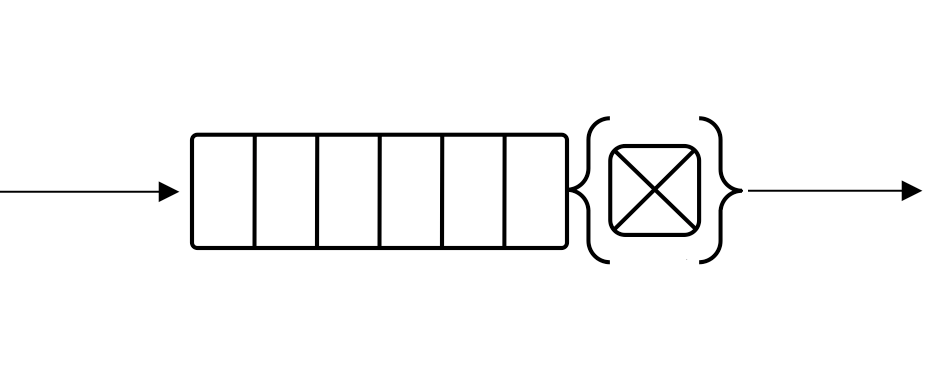
\includegraphics[width=\textwidth]{images/QSD/MM12}
                \caption{\small Single server.} 
        \end{subfigure}\qquad
        \begin{subfigure}[c]{0.40\textwidth}
                \centering
                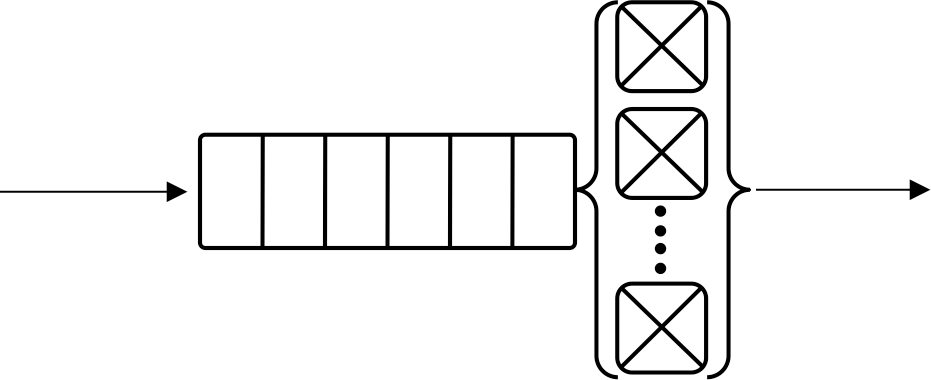
\includegraphics[width=\textwidth]{images/QSD/MMc}
                \caption{\small Parallel servers} 
        \end{subfigure}
        \begin{subfigure}[c]{0.40\textwidth}
                \centering
                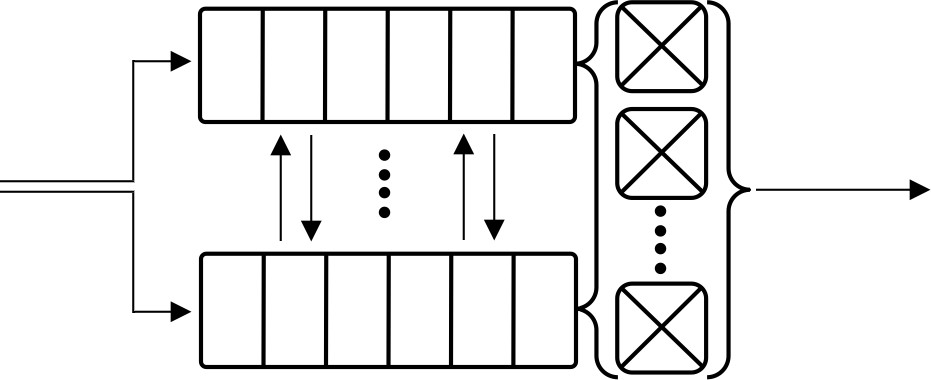
\includegraphics[width=\textwidth]{images/QSD/Tandem}
                \caption{\small Tandem queues} 
        \end{subfigure}\caption{\small Possible service facilities.} \hrule
\label{fig:service_facilities}
\end{figure}
\subsubsection{Notes, Challenges and Pitfalls}
\begin{itemize}[noitemsep]
\item Applications have mostly been concerned with the \textbf{busy period} (starting with the arrival of a customer in an empty queue and ending once the queue is empty again), and with the distribution of \textbf{waiting times}, as these are often the concepts for which improvement (or the ability to control) is sought. 
\item \textbf{Performance measures} are useful to investigate and describe the behaviour of a queueing system. They can include the mean and variance (or the full distribution) of the minimum and/or variance of the: 
\begin{enumerate}
\item number of customers;
\item waiting times;
\item service times;
\item length of busy periods;
\item delay;
\item etc.
\end{enumerate}
\item Some queueing systems have been more thoroughly studied, either because of their historical importance and simplicity, or because the model a wider range of queueing behaviour.  
\begin{description}
\item[$M/D/1$:] queue  with a single server, where arrivals are determined by a Poisson process and  service times are fixed. \item[$M/D/c$:] queue with $c$ servers, where arrivals are determined by a Poisson process and  service times are fixed.
\item[$M/M/1$:] queue with a single server, where arrivals are determined by a Poisson process with mean $\lambda$ and  service times follow an exponential distribution with mean $\frac{1}{\mu}$. 

\item[$M/M/c$:] queue with $c$ servers, where arrivals are determined by a Poisson process with mean $\lambda$ and  service times follow an exponential distribution with mean $\frac{1}{\mu}$.
\item[$M/G/1$:] queue with a single server, where arrivals are determined by a Poisson process and service times follow a general distribution.
\item[$M/G/k$:] queue with $k$ servers, where arrivals are determined by a Poisson process and service times follow an arbitrary distribution.
\item[$G/G/1$:] queue with a single server, where arrivals are determined by an arbitrary distribution and service times follow another arbitrary distribution.
\item[$G/G/k$:] queue with $k$ servers, where arrivals are determined by an arbitrary distribution and service times follow another arbitrary distribution.
\end{description}
\item The $M/M/1$ model is one of the simplest queues to analyze, and as such a lot of its performance measures can be computed explicitly. Let $\lambda$ be the mean arrival rate, and $\frac{1}{\mu}$ be the mean service time, then:
\begin{enumerate}
\item the queue is \textbf{stable} only if $\lambda<\mu$;
\item the busy period is characterized by mean $(\mu-\lambda)^{-1}$ and variance $\left(1+\frac{\lambda}{\mu}\right)\cdot\mu^{-2}\cdot \left(1-\frac{\lambda}{\mu}\right)^{-3}$;
\item the probability that a passenger has to wait upon entering the queue is $\frac{\lambda}{\mu}$;
\item the probability that a passenger will have to wait $x$ units of time or less before exiting the queue is $$p(x)=P(W_q\leq x)=1-\frac{\lambda}{\mu} e^{-(\mu-\lambda)x};$$
\item the \textbf{average wait time} is $\overline{W}_q=\frac{\lambda/\mu}{\mu-\lambda}$ (the full distribution depends on the queue's discipline);
\item if the service rate is unknown but the average wait time $\overline{W}_q>0$ can be computed by some other mean (possibly by using empirical data), then it is possible to recover $\mu$ from the last equality $$\mu=\frac{\overline{W}_q\lambda+\sqrt{\overline{W}_q^2\lambda^2+4\overline{W}_q\lambda}}{2\overline{W}_q}.$$
\end{enumerate}
\item The $M/M/c$ model is an extension of the $M/M/1$ model and some of its performance measures can also be computed explicitly. Let $\lambda$ and $\mu$ be as above, then:
\begin{enumerate}
\item the queue is stable only if $\lambda<c\mu$;
\item the probability that a passenger has to wait upon entering the queue is $$C(c,c\rho)=\frac{\left( \frac{(c\rho)^c}{c!}\right) \left(
\frac{1}{1-\rho} \right)}{\sum_{k=0}^{c-1} \frac{(c\rho)^k}{k!} +
\left( \frac{(c\rho)^c}{c!} \right) \left( \frac{1}{1-\rho}
\right)},$$ where $\rho=\frac{\lambda}{c\mu}$ is the \textbf{traffic intensity};
\item the average number of customers in the system is $\frac{\rho}{1-\rho} C(c,c\rho) + c \rho$;
\item if the queue's discipline is \textbf{work-conserving}, the average time spent in the system is $$\frac{C(c,c\rho)}{c \mu - \lambda} + \frac{1}{\mu}.$$
\end{enumerate}
\item Other queueing models are not understood to the same extent, and their given performance measurements may only be approximative and highly-dependent on the specifics of the problem at hand. For this reason, $M/M/c$ models are sometimes used even when their use is not supported by the data (the situation is not unlike the wide use of the normal distribution). In various applications, the empirical distributions of arrivals and service times are nearly Poisson and exponential, respectively, so that the assumption is not entirely missing the mark, but numerical simulations should not be eschewed when departures from the $M/M/c$ model are too pronounced.    
\item Other key concepts of queueing theory include
\begin{description}
\item[Lindley's Equation] which can be used to model the queue's length;
\item[Little's Law] is a strong results on general queueing models which links the long-term average number of customers in a stable system to the product of the long-term average arrival rate and the average time a customer spends in the system;
\item[Klingman's Formula] is a fairly robust approximation of the average waiting time $$ \overline{W}_q \approx \left( \frac{\rho}{1-\rho} \right) \left( \frac{c_a^2+c_s^2}{2}\right) \tau,$$ where $\rho$ is the queue's \textbf{utilization},  $\tau$ is the \textbf{mean service time} and $c_a$ and $c_s$ are the coefficients of variation for arrivals and service times, respectively. 
\item[Burke's Theorem:] for an $M/M/c$ queue in a stable state, the arrival process and the departure process are modeled by the same Poisson process, which allows for the estimation of arrivals when only the departures are available, and \textit{vice-versa}.  
\end{description}

\end{itemize}
